\documentclass[a4paper, 10pt]{article}
\usepackage{standart-header}
\fancyhead[R]{Винер Даниил. БЭАД232}
\fancyfoot [C] {\thepage}
\usepackage{pgfplots}
\usepackage{pgfplots}  % Для случайной генерации чисел
\setlength{\parindent}{15pt}
\setlength{\parskip}{2mm}
\fancyhead[L]{Математический анализ—2. Семинар—1}
\renewcommand{\d}[1]{\text{d}#1}

\begin{document}
\section*{Задание №3}
Имеется компакт $D$, край которого задан уравнениями
\begin{equation*}
    \begin{cases}
        y^2=2x\\
        y=4-x\\
        y=12-x
    \end{cases}
\end{equation*}

Требуется вычислить $\displaystyle\iint\limits_{D}(x+y)\d{x}\d{y}$

Есть два варианта изобразить график на плоскости: с помощью линий уровня или плотностью точек. Воспользуемся вторым
\begin{equation*}
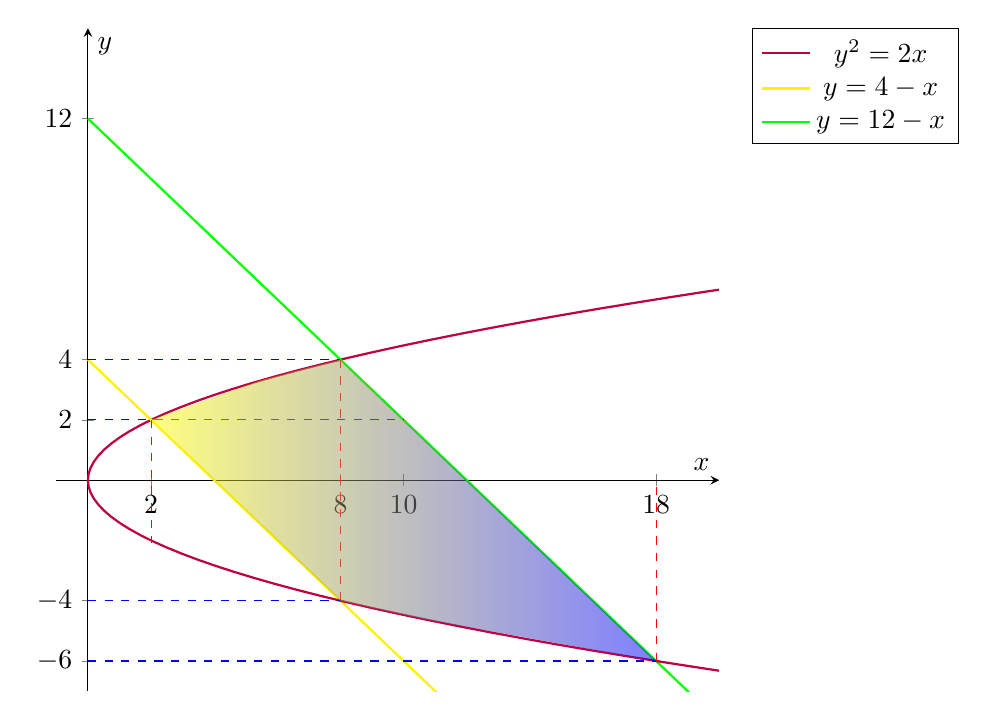
\begin{tikzpicture}
    \begin{axis}[
        axis lines=middle,          % Рисуем оси
        xmin=-1, xmax=20,           % Ограничиваем область по оси x
        ymin=-7, ymax=15,           % Ограничиваем область по оси y
        xlabel={$x$}, ylabel={$y$}, % Подписи осей
        domain=0:20,                % Область определения функции по x
        samples=100,                % Количество точек для графика
        restrict y to domain=-10:17, % Ограничиваем y для отображения графика
        ytick={-6,-4,0,2,4,12}, % Стандартные отметки + ордината 4
        minor y tick num=1,          % Промежуточные деления
        xtick={0, 2, 8, 10, 18}, % Стандартные отметки + ордината 4
        minor x tick num=1,
        width=10cm, % Ширина осей
        height=10cm, % Высота осей
        legend style={
            at={(1.05,1)}, % Позиция легенды
            anchor=north west, % Привязка легенды к указанной позиции
        }
        ]

        % Параметрический график для обеих частей (верхняя ветвь y^2=2x)
        \addplot[purple, thick, label={$y^2=2x$}] ({x^2/2}, {x});
        % Линия y = 4 - x
        \addplot[yellow, thick, label={$y=4-x$}] {4 - x};
        % Линия y = 12 - x
        \addplot[green, thick, label={$y=12-x$}] {12 - x};
         % Параметрический график для обеих частей (нижняя ветвь y^2=2x)
        \addplot[purple, thick, label={$y^2=x$}] ({x^2/2}, {-x});

        % Прямая, соединяющая точки (0,4) и (8,4)
        \addplot[blue, thin, dashed, label={$y=4$, $0 \leq x \leq 8$}] coordinates {(0,4) (8,4)};
        \addplot[blue, thin, dashed] coordinates {(0,-4) (8,-4)};
        \addplot[blue, thin, dashed] coordinates {(0,2) (10,2)};
        \addplot[blue, thin, dashed] coordinates {(0,-6) (18,-6)};
        \addplot[red, thin, dashed, label={$x=2$}] coordinates {(2,2) (2,-2.08)};
        \addplot[red, thin, dashed, label={$x=8$}] coordinates {(8,4) (8,-4)};
        \addplot[red, thin, dashed, label={$x=18$}] coordinates {(18,-6) (18,0)};

        % Определяем область для заливки градиентом
        \addplot [
            domain=0:8,                % Ограничиваем область по оси x
            samples=100,               % Количество точек для градиента
            fill=none,                 % Заливка по умолчанию
            draw=none,                 % Без границы
            left color=yellow,         % Цвет слева (начало градиента)
            right color=blue,          % Цвет справа (конец градиента)
            fill opacity=0.5,          % Прозрачность градиента
            % label={Gradient Area}      % Метка для градиента
        ]
        coordinates {(2,2) (8,-4) (10.60762,-4.606) (18,-6) (8,4) (7.0688,3.76) (5.445,3.3) (2,2)};
        
        % Легенда
        \legend{$y^2=2x$, $y=4-x$, $y=12-x$}
        
    \end{axis}
\end{tikzpicture}
\end{equation*}

Здесь и далее градиент от желтого к синему означает увеличение плотности точек в области

Чтобы вычислить интеграл, нам нужно <<нарезать>> график по осям $Ox$ и $Oy$. Синие пунктирные линии показывают \textit{горизонтальную} нарезку, а красные — \textit{вертикальную}

\subsection*{Рассмотрим горизональную нарезку}
Горизонтальная нарезка означает, что мы меняем $x$ при каких-то фиксированных $y$. Ясно, что у нас имеется всего \textbf{три} области, в которых мы будем менять переменную: $\left[-6;-4\right],\ \left[-4;2\right],\ \left[2;4\right]$, тогда искомый интеграл представим в виде:
\begin{equation*}
    \iint\limits_{D}(x+y)\d{x}\d{y}=\underbrace{\int_{-6}^{-4}\int_{\frac{y^2}{2}}^{12-y}(x+y)\d{x}\d{y}}_{I_1}+\underbrace{\int_{-4}^{2}\int_{4-y}^{12-y}(x+y)\d{x}\d{y}}_{I_2}+\underbrace{\int_{2}^{4}\int_{\frac{y^2}{2}}^{12-y}(x+y)\d{x}\d{y}}_{I_3}
\end{equation*}
\begin{equation*}
    \begin{aligned}
        I_1&=\int_{-6}^{-4}\left.\left(\frac{x^2}{2}+xy\right)\right\vert^{x=12-y}_{x=\frac{y^2}{2}}\d{y}\\
        &=\int_{-6}^{-4}\left(\left(\frac{(12-y)^2}{2}+(12-y)y\right)-\left(\frac{y^4}{8}+\frac{y^3}{2}\right)\right)\d{y}\\
        &=\int_{-6}^{-4}\left(72 - \frac{y^2}{2} - \frac{y^4}{8}-\frac{y^3}{2}\right)\d{y}\\
        &=\left.\left(72y-\frac{y^3}{6}-\frac{y^5}{40}-\frac{y^4}{8}\right)\right\vert^{-4}_{-6}\\
        &=\frac{1198}{15}
    \end{aligned}
\end{equation*}
Аналогичные вычисления производятся с интегралами $I_2,I_3$, после чего складываем и получаем результат
\subsection*{Рассмотрим вертикальную нарезку}
% Областей, в которых мы будем менять $y$ при каких-то фиксированных $x$ в данном случае \textbf{две}: 
\begin{equation*}
    \iint\limits_{D}(x+y)\d{y}\d{x}=\int_{2}^{8}\int_{4-x}^{\sqrt{2x}}(x+y)\d{y}\d{x}+\int_{8}^{16}\int_{-\sqrt{2x}}^{12-x}(x+y)\d{y}\d{x}
\end{equation*}
Заметим, что теперь во внутреннем интеграле стоит интегрирование по $y$, потому что мы делаем вертикальную нарезку


\section*{Задание №4a}
Напомним, что $\int e^{-x^2}\d{x}$ называется \textit{неберущимся}

Дан интеграл $\displaystyle\int_{0}^{1}\d{y}\int_{0}^{1-y} e^{-x^2+2x+1}\d{x}$

Пусть $\int_{0}^{1}\d{y}\int_{0}^{1-y} e^{-x^2+2x+1}\d{x}-\int_{0}^{1}\d{x}\int_{0}^{1-y} e^{-x^2+2x+1}\d{y}=I$, тогда

\begin{minipage}{0.5\textwidth}
    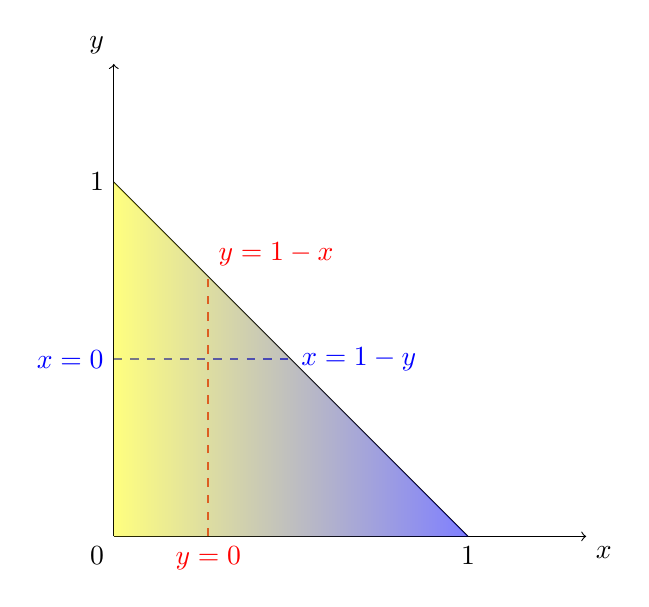
\begin{tikzpicture}[scale=1.5]
        \draw[black, ->] (0,0) node[below left] {$0$} -- (0,4) node[above left] {$y$};
        \draw[black, ->] (0,0) -- (4,0) node[below right] {$x$};
        \draw[black] (0,3) node[left] {$1$} -- (3,0) node[below] {$1$};
    
        \draw[dashed, thick, red] (0.8,0) node[below] {$y=0$} -- (0.8,2.2) node[above right] {$y=1-x$};
        \draw[dashed, thick, blue] (0,1.5) node[left] {$x=0$} -- (1.5,1.5) node[right] {$x=1-y$};
    
    
        \shade[left color=yellow, right color=blue, opacity=0.5] 
                (0,0) -- (0,3) -- (3,0) -- cycle;
    \end{tikzpicture}
\end{minipage}
\begin{minipage}{0.5\textwidth}
\begin{equation*}
    \begin{aligned}
        I&=\int_0^1\d{x}\left.e^{-x^2+2x+1}\right\vert^{1-x}_{y=0}\\
        &=\int_0^1 e^{-x^2+2x+1}(1-x)\d{x}-0\\
        &=\int_0^1-e^{-(x-1)^2+2}(1-x)\d{(x-1)}\\
        &\text{пусть $x-1=t$, тогда $\d{t}=\d{(x-1)}$}\\
        &=\int_{-1}^0 -e^{-t^2+2}t\d{t}\\
        &=\int_{-1}^0 e^{-t^2}e^{2}(-t)\d{t}\\
        &=\int_{-1}^{0} -2te^{-t^2}\cdot\frac{1}{2}e^2\d{t}\\
        &=\left.\frac{1}{2}e^2(e^{-t^2})\right\vert^{t=0}_{t=-1}\\
        &=\frac{1}{2}e(e-1)
    \end{aligned}
\end{equation*}
\end{minipage}

\section*{Задание №2a}
Дан двойной интеграл: $\displaystyle\int_0^6\d{x}\int_{\frac{x^2}{6}-1}^{x-1}f(x,y)\d{y}$

Чтобы изменить порядок интегрирования взглянем на левый интеграл. Видим, что мы меняем $x$, а границы образованы точками пересечения графиков. Значит, чтобы изменить интегрирование на $y$ возьмем ординаты точек пересечения

В правом интеграле нужно просто выразить $x$ через $y$

\begin{tikzpicture}
    % Настройки осей
    \draw[->] (-1,0) -- (7,0) node[right] {$x$};
    \draw[->] (0,-2) -- (0,7) node[above] {$y$};
    \draw[dashed, blue, thick] (-1,-1) -- (7,-1);
    \draw[dashed, blue, thick] (-1,5) -- (7,5);
    \draw[dashed, black, thin] (6,5) -- (6,0);

    \node[below left] (0,0) {$0$};

    % Парабола y = x^2/6 - 1
    \draw[domain=-1:7,smooth,variable=\x,green, thick] 
        plot ({\x},{(\x*\x)/6 - 1}) 
        node[above] {$y = \frac{x^2}{6} - 1$};

    % Прямая y = x - 1
    \draw[domain=-1:7,smooth,variable=\x,red, thick] 
        plot ({\x},{\x - 1}) 
        node[right] {$y = x - 1$};
    
    % Отметки на осях
    \foreach \x in {1,2,3,4,5,6}
        \draw (\x,1pt) -- (\x,-3pt) node[below] {$\x$};
    \foreach \y in {-1,1,2,3,4,5,6}
        \draw (1pt,\y) -- (-3pt,\y) node[left] {$\y$};
\end{tikzpicture}

Таким образом, получим, что $\displaystyle\int_0^6\d{x}\int_{\frac{x^2}{6}-1}^{x-1}f(x,y)\d{y}=\displaystyle\int_{-1}^{5}\d{y}\int_{y+1}^{\sqrt{6y+6}}f(x,y)\d{x}$

\section*{Задание №4b}
Заметим, что $x$ является константой относительно $y$ в правом интеграле, поэтому можем внести $x$ в интеграл по $\d{y}$, тогда получим:

\begin{minipage}{0.5\textwidth}
\begin{equation*}
    \begin{aligned}
        \int_0^\pi x\d{x}\int_x^\pi\frac{\sin y}{y}\d{y}&=\int_0^\pi x\int_x^\pi\frac{\sin y}{y}\d{y}\d{x}\\
        &=\int_0^\pi \int_x^\pi x\frac{\sin y}{y}\d{y}\d{x}\\
        &=\int_0^\pi \int_0^y x\frac{\sin y}{y}\d{x}\d{y}\\
        &=\int_0^\pi \frac{\sin y\cdot y}{2}\d{y}\\
        &=\frac{\pi}{2}
    \end{aligned}
\end{equation*}
\end{minipage}
\begin{minipage}{0.5\textwidth}
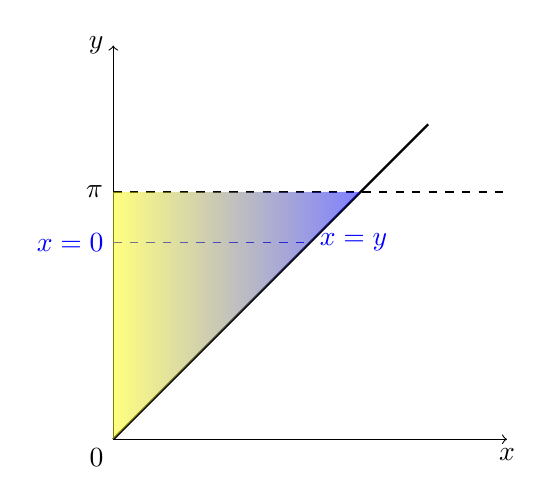
\begin{tikzpicture}
    \draw[black, ->] (0,0) -- (0,5) node[left] {$y$};
    \draw[black, ->] (0,0) -- (5,0) node[below] {$x$};
    \draw[black, thick] (0,0) -- (4,4);
    \draw[black, dashed, thick] (0,3.1415926) node[left] {$\pi$} -- (5,3.1415926);
    \draw[blue, dashed] (0,2.5) node[left] {$x=0$} -- (2.5,2.5) node[right] {$x=y$};

    \node[below left] (0,0) {$0$};
    % \node[left] (0, 3.1415926) {$\pi$};
    % \node[below, left] (0,0) {$0$};

    \shade[left color=yellow, right color=blue, opacity=0.5] 
                (0,0) -- (0,3.1415926) -- (3.1415926,3.1415926) -- cycle;
   
\end{tikzpicture}
\end{minipage}





\end{document}